\chapter{Introduction}
\label{cha:intro}

\epigraph{The best weapon of a dictatorship is secrecy, but the best weapon of a democracy should be the weapon of openness.} 
{\textit{Niels Bohr}} 

\section{Problem Statement}
   Electronic voting is a nightmare because the minuscule possibility of 
   a bug in software used in voting could lead to a disaster, possibly 
   inverting the results
   \footnote{https://people.eng.unimelb.edu.au/vjteague/UniversalVerifiabilitySwissPost.pdf}
   \citep{Wolchok:2010:SAI:1866307.1866309},
   \citep{10.1007/978-3-319-22270-7_3}, \citep{ARANHA2019335},
   \citep{Feldman:2007:SAD:1323111.1323113}.
   Given that the risk of  electronic voting is 
   so high, we should totally refrain from it. However,
   electronic voting is getting popular in many countries
   despite the fact that 
   electronic voting has many undesirable problems.  The reason that 
   electronic voting is getting popularity in many countries is cost-effective, 
   increase in voter turnout  and faster result.  India has 900 million eligible voter, 
   and with 67 percent (roughly 600 million) voter turnout in 2019 general election, 
   the result was declared in 2 days. This was possible because India uses  electronic 
   voting machines (EVM) to conduct the election. Australia has 
   compulsory voting, but its massive size with sparsely populated land makes 
   the election a big logistic challenge.  Australia is actively pursuing Internet voting 
   to ease the logistic challenges and engage more citizens from the remote places. Estonia
   is praised for successfully implementing the Internet voting since 2005. The first country to
   adopt internet voting and showing confidence in technology. In 2019 elections, 
   as claimed on e-estonia \footnote {https://e-estonia.com/solutions/e-governance/i-voting/},
   the time saved was 11,000 working days. 
  
   
   It seems that electronic voting is a silver bullet and solution to many problems, and 
   we can safely ignore the problems posed by it.   It is a worthwhile discussion that 
   what a democracy want? A faster, but wrong and unverifiable result, or a slower, but
   correct and verifiable result.  By its inherent nature, electronic voting has many 
   problems, which are not present in paper ballot election, that makes it perfectly susceptible 
   to delivering wrong and unverifiable result.
   Because of the  untrusted and complex software
    \footnote{Unix operating system has 15 million code which can not trusted at all}
    and hardware stack
 \footnote{Intel has many undocumented instructions in its x86 
 processor. https://github.com/xoreaxeaxeax/sandsifter}, 
   electronic voting lacks:  
   \begin{enumerate}
   \item correctness, i.e. produced results are correct and convincing to everyone leaving 
   no ground for suspicion.
   \item privacy,  i.e.  protecting the identity of the voter of a cast ballot
   and the choices on the cast ballot.
   \item verification, i.e. any independent observer  can establish/verify
    the produced results are correct based on cast ballots. 
   
   
   \end{enumerate}
   
	\noindent
	The software and hardware used in the electronic voting process  
	are treated as a black-box which  violates the 
	fundamental property of  public examinability. Also, they 
	expose a attack surface
	which  could potentially be exploited for illegal gain in election, possibly by 
	current government or foreign country. As a result, a person who has 
	not legitimately received a majority or quota would be  put in charge of public office. 
	In a  nutshell, 
    electronic voting lacks violates the  fundamental principals of any democratic election, i.e.
    correctness, privacy, and verifiability. 
 	

\section{Research Motivation and Contribution}
Given the potential advantages of electronic voting,  we need to address
the correctness, privacy and verifiability concerns for its widespread adoption. 
This thesis sets out to address these concerns of electronic voting. 
The questions we asked ourself was:
 \begin{enumerate} 
  \item Can we implement a vote counting protocol with the  
    guaranteed correctness of its properties, and practical enough
    to count the real life election involving millions of ballots ? (Correctness)
  \item Can we produce the result by counting encrypted ballot without revealing 
  its content, and at the same time, 
  assuring everyone that the result produced is only based on valid ballots, 
  and invalid ones have been discarded ? (Privacy)
 \item Can we decouple the verifiability from implementation, i.e. 
    generating enough evidence so that any independent auditor can 
    ascertain the outcome of election without trusting the implementation 
    of software used to conduct the election? (Verifiability)
  \end{enumerate}


We answer these question by taking \cite{Schulze:2011:NMC} 
algorithm as an example and Coq \citep{Bertot:2004:ITP}
theorem prover  for implementing and proving the correctness of  Schulze method.
Even though Schulze method is not used in any democratic election, the reason 
 we went ahead with it because it has many interesting properties and, 
 at the same time, it is non-trivial.   Schulze's method elects  a single winner based on 
preferential votes.  Arrow's impossibility theorem \citep{Arrow:1950:DCS} states
 that no preferential voting 
scheme can have all the desired properties established by  social choice theorist,
the Schulze's method offers a good balance. We will discuss more about Schulze method in 
\ref{cha:schulze_method}, and about its properties in \ref{cha:machine_checked}. 
The reason for choosing Coq is that it supports an expressive logic and dependent 
inductive types which is very crucial for us. We will discuss more about the Coq in 
\ref{cha:background}. 

We demonstrate the:
\begin{enumerate}
 \item \texttt{Correctness} by formally specifying the Schulze method  inside 
 Coq theorem prover, and prove the correctness properties. 
 Coq has a well developed extraction facility that 
 we use to extract proofs into OCaml programs, and using these extracted OCaml programs, we 
 have counted the ballots from election to produce the result. 
 \item \texttt{Verifiability} by tabulating the relevant data of election. We call it scrutiny-sheet/certificate. 
   Achieving verifiability in a plain-text ballot counting is fairly straight forward, but it is not 
   the same with encrypted ballot counting.  To achieve verifiability in encrypted ballot counting, 
   we augment the scrutiny sheet with zero-knowledge-proof for the each claim we make during the 
   counting which can  later be checked by any auditor.  
 \item \texttt{Privacy} by encryption. We use homomorphic-encryption to compute the 
  finally tally without decrypting any individual ballot. 
\end{enumerate}


In addition to this, we have also developed a formally verified certificate checker to ease the 
auditing of election conducted on encrypted ballot.  Given that our certificate is very complex 
and formalizing all primitives involved would be fairly time consuming, we have developed a 
proof of concept for IACR 2018, relatively simple than ours, election scrutiny sheet
\ref{cha:software_independence}. 
Also, we have proved couple of properties, Condercet winner, and Reversal symmetry property 
of Schulze method inside Coq theorem prover \ref{cha:machine_checked}.

\section{Cryptographic Assumption}
The goal of this thesis is not to verify the cryptographic primitives, but use them as a 
facilitator to achieve privacy and verifiability in electronic voting. To achieve it, we have 
taken the axiomatic approach, and assumed the existence of cryptographic primitives 
inside Coq theorem prover with the 
axioms about their correctness behaviour. These primitives, in general, provide functionality 
of encrypting a plain-text, decrypting a cipher-text, constructing a zero-knowledge-proof, 
and verifying a zero-knowledge-proof. Later, in extracted OCaml, these functions are instantiated 
with some external library function.  We will discuss more on this in \ref{cha:homormorphic_schulze}.
\footnote{Formalizing the whole cryptographic stack used in our 
project would be very time consuming (probably a PhD itself), but it would be worth trying. 
Although, we have formalized the (El-Gamal) encryption, and decryption inside Coq, but we still 
are very far from achieving the goal of fully verified cryptographic stack.  We leave the formalisation 
of cryptographic primitives for future work (work in progress).}



\section{Publication}
	\begin{enumerate}
	\item Pattinson, D. and Tiwari, M., 2017. Schulze voting as evidence carrying computation. In Proc. 
	ITP 2017, vol. 10499 of Lecture Notes in Computer Science, 410–426. Springer. 
	\item Lyria Bennett Moses, Rajeev Goré, Ron Levy, Dirk Pattinson, Mukesh Tiwari:
	No More Excuses: Automated Synthesis of Practical and Verifiable Vote-Counting Programs for Complex 
	Voting 	Schemes. E-VOTE-ID 2017: 66-83
	\item Milad K. Ghale, Rajeev Goré, Dirk Pattinson, Mukesh Tiwari:
	Modular Formalisation and Verification of STV Algorithms. E-Vote-ID 2018: 51-66
	\item VSSTE paper
	\item CCS paper

	\end{enumerate}




\section{Related Work}
 There are extensive work which 
 addresses the different issues related of electronic voting protocols  in symbolic model, 
 but there are very few, to the best of my knowledge, 
 which has used theorem prover to implement the voting protocol (counting algorithm)
 and verify its correctness properties. 
 \cite{10.1007/978-3-540-31987-0_14}, and  \cite{Delaune2010} have used pi-calculus to model 
 and analyse various properties, fairness, eligibility, vote-privacy, receipt-freeness and coercion-resistant,  
 of the protocol FOO developed by \cite{10.1007/3-540-57220-1_66}.  \cite{Backes:2008:AVR:1380848.1381255}
 presented a general technique to model  remote electronic 
 voting protocol and automatically verifying  its security properties using pi-calculus. 
 \cite{5992139} have used pi-calculus to analyse the ballot secrecy of \cite{Helios:2016:HVS}.
 \cite{10.1007/978-3-642-28641-4_7} have used pi-calculus to ascertain the properties of 
 Norwegian electronic voting protocol.
 \cite{10.1007/978-3-319-68687-5_7} have used Tamarin  to prove receipt-freeness 
 and vote-privacy of Selene voting protocol \citep{Selene}.  Most of these work differs from ours
 in the sense that their primary focus is verification of security protocol in  
 Dolev-Yao model or  complexity-theoretic model, whereas our work is 
 more focused on verified implementation and  verifiability  aspect of election.

 The closest to our work is \cite{DeYoung:2012:LLV}, \cite{Pattinson:2015:VCM}, \cite{Pattinson:2016:MSP},
 \cite{Verity:2017:FVI:3014812.3014845}, and \cite{Ghale:2017:FVS}.  \cite{DeYoung:2012:LLV} 
 used linear logic\citep{GIRARD19871} to model the different entity in electronic voting as a resource. 
 The use of linear logic makes it very natural to capture the different entities in electronic voting,  
 depending on their usage, by means of modality e.g. a voter can cast only one vote, but he might 
 need to show his photo id to multiple times at counting booth. \cite{Pattinson:2015:VCM} treated 
 the process of vote counting from
 the perspective of mathematical proof. They used (mathematical) proof theory to model the 
 counting. \cite{Ghale:2017:FVS} have formalized the single transferable votes in Coq and 
 extracted a Haskell code from the formalization. The extracted Haskell code produces the result 
 and a certificate for a given set of input ballots. The certificate can be used by any third party to verify 
 or audit the outcome of election result.  However, none of these work considers privacy as a key 
 issue in electronic voting, and their method simply works for plaintext ballots which are  susceptible to 
 "italian attack"  \citep{Otten}   \citep{Benaloh:2009:SSC}.

\section{Outline of the Chapters}
[Rewrite again when you finish everything]
In chapter 2, we will give a brief history of electronic voting, the glitches that cause some countries 
to withdraw from electronic voting.  



\section{Trivia}
 Before 1856, Victoria and NSW held their elections to elect its 
	  democratic representative in pub where it was legal for 
	  candidates to offer beer to voters to influence their 
	  decision! 
	  
	   \begin{figure}[htb]
	\begin{center}
	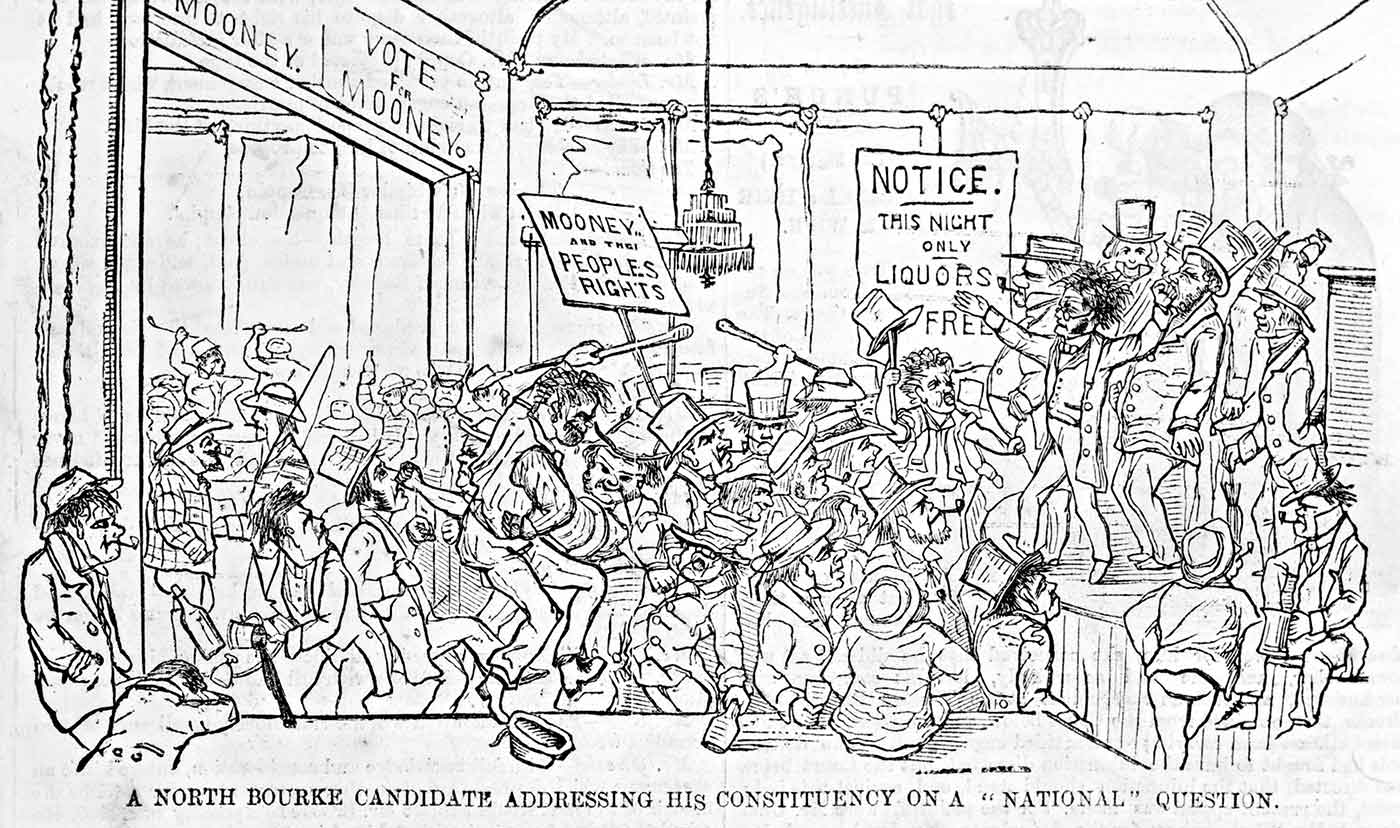
\includegraphics[scale=0.25]{NorthBourke.jpg}
	\caption{Election held in 1855 in Victoria, Australia 
	  was conducted in pub!}
	\end{center}
  \end{figure}   
  
  







A democracy can be best describe as a system where every participant 
has equal right to express his opinion(s) on different matters. Each
eligible participant expresses his opinion, and a winner is elected 
by using some method to combine every participant's opinion.
In current context of democratic elections, 
every eligible participant expresses his opinion on a paper, also 
known as ballot, 
by marking a tick against the preferred candidate 
(first-past-the-post) or ranking the candidates in some order
(preferential voting). 
One of the most fundamental assumption during any democratic 
election, privacy and anonymity about the voter's choices, was not the case 
in past. It was Victoria, Australia who first introduce the 
concept of secret ballot in 1856 \footnote{
 https://trove.nla.gov.au/work/25532676?q\&versionId=30761831}
 \footnote{https://www.nma.gov.au/defining-moments/
	  resources/secret-ballot-introduced} and gradually, it 
	  got adoption all over the world. Before 1856, Victoria
	  and NSW held their elections to elect its 
	  democratic representative in pub where it was legal for 
	  candidates to offer beer to voters to influence their 
	  decision! 
	  
Verifiability or transparency is other fundamental assumption for 
any democratic election. Transparency insures that each step of 
of election process is easily understood and can be scrutinize by 
every stake holders e.g. voters, political parties, and external 
observers. Privacy and verifiability  are basic 
ingredient for coercion free election, i.e. people 
can express their opinion with any concern, and at the same time,
they can not sell their votes. Without privacy and verifiability, 
we can not expect a true democracy.   

 
 \begin{figure}[htb]
	\begin{center}
	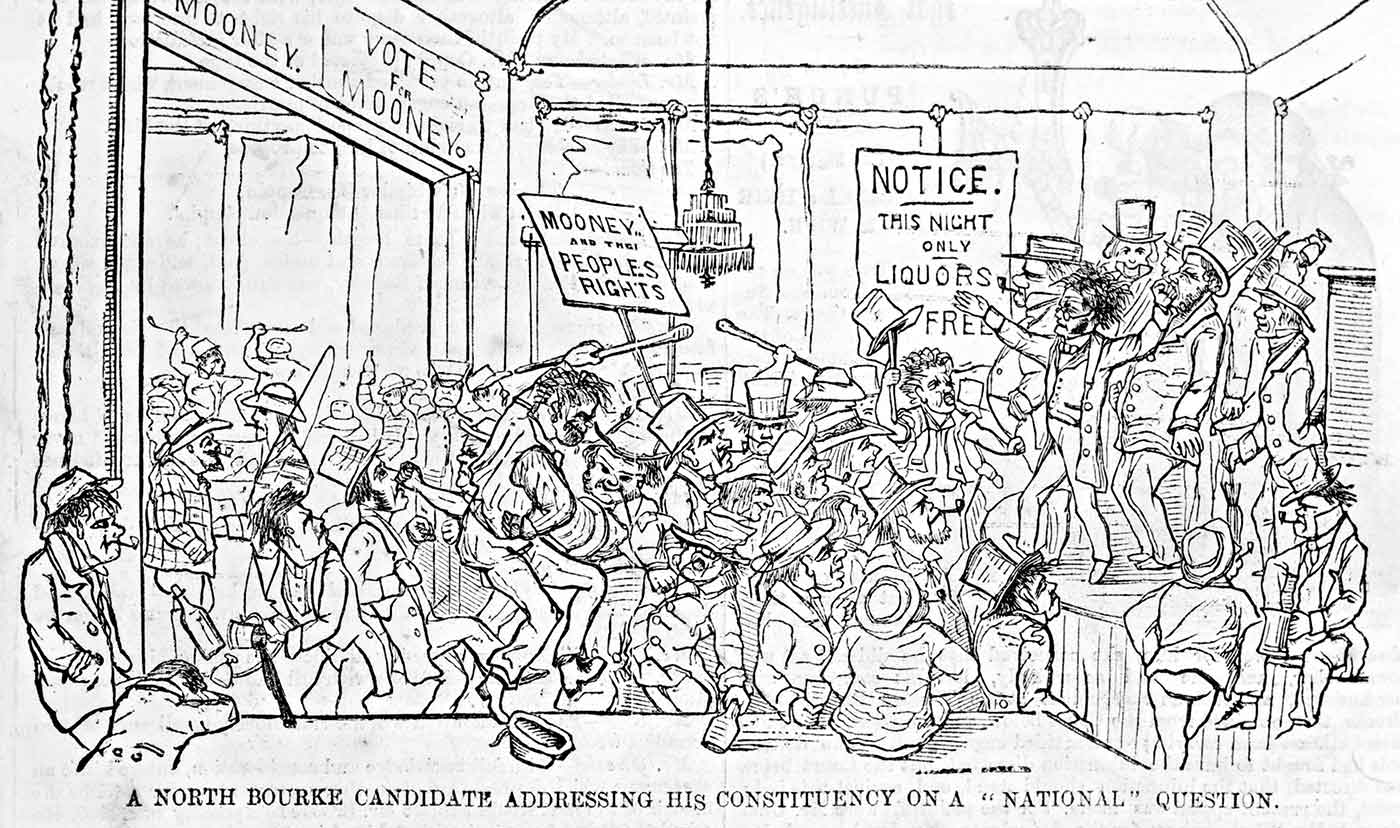
\includegraphics[scale=0.25]{NorthBourke.jpg}
	\caption{Election held in 1855 in Victoria, Australia 
	  was conducted in pub!}
	\end{center}
  \end{figure}   
  
 Electronic voting is very different from paper ballot election. 
 Reasoning 
 about privacy and verifiability and many other properties 
 in paper ballot election 
 is straight forward, but we can not do the same for 
 electronic voting election. The reason is, electronic voting constitutes 
 of various untrusted component of software
 \footnote{Unix operating system has 15 million code which can not 
 trusted at all} and hardware
 \footnote{Intel has many undocumented instructions in its x86 
 processor. https://github.com/xoreaxeaxeax/sandsifter} which 
 exposes a large attack surface. These attack surfaces could 
 potentially be exploited for illegal gain in election. 
 Even though electronic voting is gaining popularity, none so far has 
 addressed the software bug issue in electronic voting context. 
 Most of the software used in electronic voting process are 
 inadequately tested which evidently can not rule out all 
 the possibilities.
  
 \section{Motivation and Research Statement}
 \textbf{Motivation:}
 Electronic voting has gained a lot of attention in recent year,  and  there are extensive work which 
 addresses the different issues related of electronic voting protocols  in symbolic model.
% , 
% but there are very few, to the best of my knowledge, 
% which has used theorem prover to implement the voting protocol (counting algorithm)
% and verify its correctness properties. 
 \cite{10.1007/978-3-540-31987-0_14}, and  \cite{Delaune2010} have used pi-calculus to model 
 and analyse various properties, fairness, eligibility, vote-privacy, receipt-freeness and coercion-resistant,  
 of the protocol FOO developed by \cite{10.1007/3-540-57220-1_66}.  \cite{Backes:2008:AVR:1380848.1381255}
 presented a general technique to model  remote electronic 
 voting protocol and automatically verifying  its security properties using pi-calculus. 
 \cite{5992139} have used pi-calculus to analyse the ballot secrecy of \cite{Helios:2016:HVS}.
 \cite{10.1007/978-3-642-28641-4_7} have used pi-calculus to ascertain the properties of 
 Norwegian electronic voting protocol.
 \cite{10.1007/978-3-319-68687-5_7} have used Tamarin  to prove receipt-freeness 
 and vote-privacy of Selene voting protocol \citep{Selene}.  Most of these work differs from ours
 in the sense that their primary focus is verification of security protocol in  
 Dolev-Yao model or  complexity-theoretic model, whereas our work is 
 more focused on verified implementation and  verifiability  aspect of election.
[Note to myself: Carsten has used the term "auditable correctness of implementations" for this]
 
 The closest to our work is \cite{DeYoung:2012:LLV}, \cite{Pattinson:2015:VCM}, \cite{Pattinson:2016:MSP},
 \cite{Verity:2017:FVI:3014812.3014845}, and \cite{Ghale:2017:FVS}.  \cite{DeYoung:2012:LLV} 
 used linear logic\citep{GIRARD19871} to model the different entity in electronic voting as a resource. 
 The use of linear logic makes it very natural to capture the different entities in electronic voting,  
 depending on their usage, by means of modality e.g. a voter can cast only one vote, but he might 
 need to show his photo id to multiple times at counting booth. \cite{Pattinson:2015:VCM} treated 
 the process of vote counting from
 the perspective of mathematical proof. They used (mathematical) proof theory to model the 
 counting. \cite{Ghale:2017:FVS} have formalized the single transferable votes in Coq and 
 extracted a Haskell code from the formalization. The extracted Haskell code produces the result 
 and a certificate for a given set of input ballots. The certificate can be used by any third party to verify 
 or audit the outcome of election result.  However, none of these work considers privacy as a key 
 issue in electronic voting, and their method simply works for plaintext ballots which are  susceptible to 
 "italian attack"  \citep{Otten}   \citep{Benaloh:2009:SSC}.
 
 This work not only considers the plaintext ballot, but extends the counting to encrypted ballot 
 using homomorphic encryption to preserve the privacy of election. To ensure the verifiability, 
 we use the zero-knowledge-proof to 
 make sure that outcome of election can be attested by any independent third party. To ease the 
 auditing or certificate-checking of election conducted on encrypted ballot with other complex 
 cryptographic entities, we have developed 
 a formally verified certificate checker for auditing the election \footnote{IACR 2018 election}. 
 To the best of our knowledge, no one has developed a vote counting system which counts encrypted 
 ballots, and at the same time, the implementation itself is verified inside a theorem prover.  
 \citep{10.1007/978-3-030-03592-1_5} has developed a verified certificate checker, but, again, 
 it involves plaintext ballots  with simple mathematics of addition and multiplication while  our checker
 tackles the certificates involving complex cryptographic 
 objects, e.g. encrypted ballots and zero-knowledge-proof of different statements.
 
 
\textbf{Research Statement:}
After inspecting the current state of art in electronic voting, we 
 asked ourselves three questions:
 \begin{enumerate}
  \item Can we engineer a system which is formally verified to 
    guarantee the correctness property, and practical enough
    to count the real life election involving millions of ballots ? 
 \item  Can we decouple the verifiability from implementation, i.e. 
    generating enough evidence so that any independent auditor can 
    ascertain the outcome of election without trusting the implementation 
    of software used to conduct the election ? 
  \item How "good"  is our proposed solution ?
  \end{enumerate}
  
  
 In order to answer these three questions, we needed three things:
\begin{enumerate}
  \item A voting protocol
  \item A theorem prover to implement the voting protocol
  \item Parameters, agreed upon properties in electronic voting research community, against which 
  		  we will measure our solution
\end{enumerate} 
 
 \subsection{Voting Protocol}
 For voting protocol, we settled down with \cite{Schulze:2011:NMC}.
 Even though Schulze method is not used in any democratic election, the reason 
 we went ahead with it because it is interesting  and at the same time, non-trivial. 
 Schulze's method elects  a single winner based on 
preferential votes.  At the same time, Arrow's impossibility theorem \citep{Arrow:1950:DCS} states
 that no preferential voting 
scheme can have all the desired properties established by  social choice theorist,
the Schulze's method offers a good balance. Many of these properties are already 
established in his original paper.  We will discuss more about Schulze method in 
\ref{cha:schulze_method}, and about its properties in \ref{cha:machine_checked}. 

\subsection{Theorem Prover:}
Our preference for theorem prover was Coq \citep{Bertot:2004:ITP}. The 
reason for choosing Coq is that it supports an expressive logic and  (crucial for us) dependent 
inductive types.  Coq has a well developed extraction facility that 
we use to extract proofs into OCaml programs, and using these extracted OCaml programs, we 
have counted the ballots from election to produce the result.  We will discuss more about the Coq in 
\ref{cha:background}. 

\subsection{Properties of Electronic Voting Protocol:} 
 What makes a electronic voting protocol  "good" or "desirable" ?  Some commonly sought 
 properties which a electronic voting protocol must have are given below \citep{5958051}, 
 \citep{Benaloh:1994:RSE:195058.195407},  \citep{Delaune:2010:VPT}, \citep{Bernhard:2017:PES}.
 \begin{itemize}
 
  \item Correctness:
 	The produced results are correct, and convincing to all leaving no  ground for suspicion. 
 	
 \item Privacy:
    All the votes must be secret, and voter should not be able to convince anyone the 
    value of his vote.
 
 \item End-to-end Verifiability:
 Any independent third party should be able to verify the final outcome of election based on cast 
 ballots.  It can be further divided into three sub-category:
 
 \begin{itemize}
  \item Cast-as-intended: Every voter can verify that their ballot was cast as
  intended
  \item Collected-as-cast: Every voter can verify that their ballot was collected as
  cast
  \item Tallied-as-cast: Everyone can verify final result on the basis of the
  collected ballots.
\end{itemize}

\item Practicality/Usability: 
  
\item Coercion-resistance:
	A voter cannot cooperate with a coercer to prove to him that she voted in a certain way.
  
\item Voter Eligibility:
  Only eligible voter can cast the ballot, and only once.

\item Fairness:
  No intermediate results can be obtained which could influence the remaining voters.

\item Receipt-freeness:
A voter does not gain any information (receipt) which can be used to prove to a coercer that
she voted in a certain way

 \end{itemize}
 
  
 
% 
%	\begin{itemize}
%	\item Correctness : The produced results are correct, and convincing to all leaving no 
%	          ground for suspicion. 
%	\item Coercion-resistance: 
%	\item Eligibility
%	\item Fairness
%	\item Privacy
%	\item Practicality
%	\item Individual-verifiability
%	\item Universal-verifiability
%	\item Receipt-freeness
%	\end{itemize}


The focus of our study is the \textit{Correctness}, 
 \textit{Practicality}, \textit{Verifiability}, i.e. generating enough evidence so that 
 everyone can verify final result on the basis of the collected ballots, and \textit{Privacy}. In the critical 
 summary of each chapter, we will measure our solution against these properties. 
 
 
%
%\textbf{Chapter Overview}
%[Leave it till the end. Do I need chapter overview for this chapter ?]


%\section{Motivation and Problem Statement}
% \fix{What is the motivation behind this research ? Clearly state your \
%      Problem statement}
	      
%  Before I start diving deep into explaining the bits and pieces 
%  of electronic voting, Schulze method, and Coq theorem prover, 
%  I still need to persuade the reader that why this thesis 
%  exists in first place ?  Why did I choose to certify Schulze 
%  algorithm in Coq given the fact that it is not used in 
%  any democratic election and Coq is not serious business
%  in certifying the software used in electronic voting.  
%  Probably, this is the only time where I would unearth 
%  the philosopher inside me and go to length to explain 
%  the implication of my work. 
%  
  
       
%  Well, the honest answer is that  I want to graduate (hopefully), but
%  it's still not convincing argument because I could have chosen 
%  some other project and graduate. 
%%   
%  [Motivate should refer to some past research, but none of 
%  them address the problem of bugs in software.  
%  
%  On the serious note, the motivation
%  behind this thesis to find the answer of question:  
%  
%  Can we afford bugs in software used for vote counting, and 
%  can we engineer a system which has all the "desirable properties" ?
%  
%  We would answer the 
%  
    
      
 
 
%
%\section{Contribution}
%  

	\section{Publication}
	During the course of PhD, I was fortunate to work with many researchers including my supervisor 
	Dr. Dirk Pattinson, co-supervisor Rajeev Goré, colleague Milad K. Ghale,  and external collaborators 
	Dr. Thomas Haines from NTNU, Dr. Lyria Bennett Moses from UNSW, and Dr Ron Levy from ANU.  
	\begin{enumerate}
	\item Pattinson, D. and Tiwari, M., 2017. Schulze voting as evidence carrying computation. In Proc. 
	ITP 2017, vol. 10499 of Lecture Notes in Computer Science, 410–426. Springer. 
	\item Lyria Bennett Moses, Rajeev Goré, Ron Levy, Dirk Pattinson, Mukesh Tiwari:
	No More Excuses: Automated Synthesis of Practical and Verifiable Vote-Counting Programs for Complex 
	Voting 	Schemes. E-VOTE-ID 2017: 66-83
	\item Milad K. Ghale, Rajeev Goré, Dirk Pattinson, Mukesh Tiwari:
	Modular Formalisation and Verification of STV Algorithms. E-Vote-ID 2018: 51-66
	\item VSSTE paper
	\item CCS paper

	\end{enumerate}
		
	

\section{Outline of the Chapters}
[Rewrite again when you finish everything]
In chapter 2, we will give a brief history of electronic voting, the glitches that cause some countries 
to withdraw from electronic voting.  



We will evaluate our work based on the agreed upon properties of electronic voting in 
the research community.  It is privacy, verifiability and practicality. In the end of each chapter, 
we will give a critical summary of  our work and which parameter is passed successfully and which 
one it failed. 



%
%Given that I am 
%computer scientist by profession, I would not try to justify my decisions by excessive use of philosophical 
%arguments, but at this point it seems very apt to first investigate this question from philosophical point. 
%
%
%
%The answer depends on how you perceive democracy.  For a dictator, probably  bug in the 
%vote software would be a natural choice, among many others,  to rig the election. If you firmly believe 
%in democracy and democratic values, then 
%among many other things, transparency and bug freeness in vote counting software  would also be 
%in your agenda. There is no doubt that technology can play a critical role in maintaining the democratic values, 
%but assuming that it is the only factor would be a gross mistake. 
%In Azerbaijan's 2013 election, the running president Ilham Aliyev launched a iPhone app, to boost the 
%credibility of election, which enabled the citizens of Azerbaijan to 
%track the tallies as counting took place. There was just one problem. The app already showed that 
%Ilham Aliyev elected before even a ballot was counted.  In this particular case, technology merely helped in 
%surfacing the problem, but it did not do any other thing.  More often technology can be used to hide 
%the transparency of system than making it evident specially in corrupt society for personal gain. 
%
%
%Democracy is a complex system of different actors interacting with each other in certain fashion.  How to make 
%these interaction more productive and better for society, I leave this to political scientists and social scientist
%to figure out, and I stick to my job as a technology enabler.  This thesis is  my journey 
%(with my supervisor) about finding  a way to make vote counting software more robust and transparent.


%
%\section{Why Schulze ?}
%\label{sec:thesisstatement}
%Even though Schulze method is not used in any democratic election, we settled down 
%with it because it is interesting  and at the same time, non-trivial. 
% Schulze's method [cite Schulze]  elects  a single winner based on 
%preferential votes.  At the same time, Arrow's impossibility theorem [cite Arrow]  states that no preferential voting 
%scheme can have all the desired properties established by  social choice theorist,
%the Schulze's method offers a good balance. Many of these properties are already 
%established in his original paper. These properties are Non-dictatorship,  Pareto,  Monotonicity, 
%Resolvability, Independence of Clones 
%
%I will discuss some of its properties in next chapter. 
%
%
%A  quantitative  comparison of voting methods 
%[cite An Optimal Single-Winner Preferential Voting System Based onGame Theory]  also shows that 
%Schulze voting is better (in a game theoretic sense) than other, more established, systems.  The 
%Schulze Method is rapidly gaining popularity in the open software community, and It is one of the most 
%popular voting protocol over internet to elect candidates. At of 22 July 2019, Wikipedia entry on Schulze 
%method [cite Wiki entry] shows at least 70 users, and some of 
%notable users among them are Gentoo Foundation, Debian, GNU Privacy Guard (GnuPG), Ubuntu, and 
%Pirate Party in Australia, Austria, Belgium, Brazil, Germany, Iceland, Italy, 
%Netherlands, New Zealand, Sweden, Switzerland, and United States.  
%
%
%
%
%
%
%\section{Why Coq}
\label{sec:outline}
How many chapters you have? You may have Chapter~\ref{cha:background},
Chapter~\ref{cha:design}, Chapter~\ref{cha:methodology},
Chapter~\ref{cha:result}, and Chapter~\ref{cha:conc}.
